%{{{ Preamble
\documentclass[a4paper,9pt]{article}
\usepackage{anysize}
\marginsize{2cm}{2cm}{1cm}{1cm}
%\textwidth 6.0in \textheight = 664pt
\usepackage{xltxtra}
\usepackage[noend]{algpseudocode}
\usepackage{algorithm}
\usepackage{xr}
\usepackage{hyperref}
\usepackage{xunicode}
\usepackage{graphicx}
\usepackage{color}
\usepackage{xgreek}
\usepackage{multirow}
\usepackage{subfig}
\usepackage{fancyvrb}
\usepackage{minted}
\usepackage{listings}
\usepackage{enumitem}
\usepackage{framed}
\usepackage{relsize}
\usepackage{float}
%\setmainfont[Mapping=TeX-text]{DejaVu Serif}
\setmainfont[Mapping=TeX-text]{FreeSerif}
%\setmonofont{Andale Mono}
%}}}
\begin{document}
\def\thesubsection {\arabic{subsection}}

\begin{titlepage}
\begin{center}
\begin{figure}[t]
     
\includegraphics[scale=0.7]{title/ntua_logo}
\end{figure}
\begin{LARGE}\textbf{ΕΘΝΙΚΟ ΜΕΤΣΟΒΙΟ ΠΟΛΥΤΕΧΝΕΙΟ\\}\end{LARGE}
\vspace{2cm}
\begin{Large}
ΣΧΟΛΗ ΗΜ\&ΜΥ\\
Τεχνητή Νοημοσύνη\\
1\textsuperscript{η} Άσκηση\\
Ακ. έτος 2011-2012\\
\end{Large}
\vspace{5cm}
\vspace{1cm}
\begin{tabular}{l r}
\Large{Γερακάρης Βασίλης}&
\large{Α.Μ.: 03108092}\\
\Large{Λύρας Γρηγόρης}&
\large{Α.Μ.: 03109687}\\
\end{tabular}\\
\vspace{5cm}

\vfill
\large\today\\
\end{center}
\end{titlepage}



\section*{Υλοποίηση αλγορίθμου A*} \setcounter{section}{1}
%{{{ Algorithm

\subsection{Παρουσίαση προβλήματος και σκιαγράφηση λύσης}
Στην άσκηση αυτή καλούμαστε να υλοποιήσουμε τον αλγόριθμο αναζήτησης Α* με
σκοπό να οδηγηθούν με βέλτιστο τρόπο 2 ρομπότ σε ένα προκαθορισμένο σημείο
συνάντησης, αποφεύγοντας τις πιθανές συγκρούσεις.

Έχοντας ως δεδομένο ότι τα δύο ρομπότ έχουν γνώση της θέσης και του
πλάνου του άλλου ρομπότ, καθώς και πλήρη γνώση της αίθουσας, επιλέξαμε να
κάνουμε μια παρατήρηση /παραδοχή που διευκολύνει σημαντικά την δομή του
προγράμματός μας:

Αντί τα 2 ρομπότ να πραγματοποιούν τις κινήσεις/επιλογές τους εναλλάξ,
θεωρούμε, χωρίς βλάβη της γενικότητας, ότι στις συγκρούσεις το 2ο ρομπότ θα
έχει μια 'nice' συμπεριφορά, παραχωρόντας τη βέλτιστη κίνηση στο 1ο ρομπότ. Με
τον τρόπο αυτό, μπορούμε να εκτελέσουμε σειριακά τον αλγόριθμο A*, πρώτα για
το 1ο ρομπότ και στη συνέχεια για το 2ο, έχοντας ήδη δεδομένες τις κινήσεις
του 1ου.

Ο χώρος των καταστάσεων μας δίνεται ως ένα grid με Ο (στις θέσεις που
επιτρέπεται η κίνηση) και Χ (στις θέσεις όπου βρίσκονται εμπόδια). Η βασική
ιδέα πίσω από τον αλγόριθμό μας είναι ότι οι θέσεις με Χ κωδικοποιούνται ως
'-1', οι θέσεις με O με '0', ενώ η θέση στην οποία θα βρίσκεται το 1ο ρομπότ
στο k-οστό βήμα με 'k'.

Με τον τρόπο αυτό, μπορούμε να περιορίσουμε τις επιλογές του 2ου ρομπότ σε
κάθε βήμα, αναγκάζοντας το να ψάξει εναλλακτικό μονοπάτι ή να μείνει στάσιμο
γι'αυτό το βήμα (αν το συμφέρει). Καταφέρνουμε έτσι να αποφύγουμε τις πιθανές
συγκρούσεις, ενώ ταυτόχρονα δε θυσιάζουμε τη βελτιστότητα της λύσης μας.

Για την υλοποίηση του παραπάνω αλγορίθμου, επιλέχθηκε ως κατάλληλη γλώσσα η
Python, επειδή μας δίνει τη δυνατότητα να επικεντρωθούμε στα πλέον σημαντικά
κομμάτια του προβλήματος (αλγόριθμος και στρατηγική αναζήτησης), να γράψουμε
πυκνό και ευανάγνωστο κώδικα, ενώ με τη χρήση ενός extension module όπως
τo \underline{\href{http://psyco.sourceforge.net/}{Psyco}} έχουμε αντίστοιχο χρόνο
εκτέλεσης όπως αν γράφαμε σε μια γλώσσα χαμηλότερου επιπέδου.

%}}}

%{{{ Data Structures

\subsection{Επιλογή Δομών Δεδομένων}
Στην υλοποίησή μας επιλέξαμε να χρησιμοποιήσουμε λίστες από τούπλες της Python,
όπου ο κάθε κόμβος στι λίστα του A* είχε 4 στοιχεία:
\begin{enumerate}
	\item Το άθροισμα ευριστικής και κόστους (h + c)
	\item Το κόστος (c)
	\item Την τετμημένη του σημείου (x)
	\item Την τεταγμένη του σημείου (y)
\end{enumerate}

Επιπλέον, χρησιμοποιείται ένα λεξικό (dict) προκειμένου να
πραγματοποιηθεί η αναδόμηση της επιλεγμένης διαδρομής ενός ρομπότ. Τα
dictionaries είναι associative arrays, ένας τύπος αντικειμένων που μοιάζει με
λίστα, αλλά όπου σε μοναδικά κλειδιά αντιστοιχίζονται (όχι απαραίτητα
μοναδικές) τιμές.

%}}}

%{{{ Basic functions

\subsection{Βασικές συναρτήσεις-τελεστές}
Οι συναρτήσεις που σχεδιάστηκαν για την υλοποίηση του αλγορίθμου, όπως
παρατίθενται στο 8\textsuperscript{ο} κομμάτι της αναφοράς, είναι οι εξής:
\subsubsection{Ανάγνωση εισόδου}
\begin{itemize}
	\item \emph{parseUser} : Διαβάζει και ελέγχει για ορθότητα τα ορίσματα
		που δώθηκαν στο πρόγραμμα.
	\item \emph{parseInput} : Διαβάζει και αποθηκεύειτις γραμμές του αρχείου
		εισόδου
	\item \emph{fieldTranslate} : Ελέγχει την ορθότητα της εισόδου της
		κάτοψης της αίθουσας και τη "μεταφράζει" στη μορφή την οποία θα
		χρησιμοποιηθεί αργότερα.
\end{itemize}
\subsubsection{Eυριστικές μέθοδοι}
\begin{itemize}
	\item \emph{manhattanDist} : Η απόσταση manhattan, υποεκτιμητής
	\item \emph{squaredDist} : Τα τετράγωνα των αποστάσεων, υπερεκτιμητής
\end{itemize}
\subsubsection{Κυρίως σώμα του Α*}
\begin{itemize}
	\item \emph{astar} : Δέχεται σαν είσοδο την αρχική και την τελική θέση, το χώρο
		καταστάσεων, την ευρεστική συνάρτηση και τον κωδικό του robot και εκτελεί
		τον αλγόριθμο Α* μέχρι να βρεί λύση. Ανασυγκροτεί το μονοπάτι που βρήκε
		και το επιστρέφει μαζί με το πλήθος των κόμβων που εξετάστηκαν
	\item \emph{nextNodes} : Επιστρέφει μια λίστα με την τετράδα των πιθανών
		κόμβων για εξέταση γύρω από ένα σημείο.
\end{itemize}
\subsubsection{Χώρος καταστάσεων}
\begin{itemize}
	\item
	\item
	\item
\end{itemize}
\subsubsection{Controller}
\begin{itemize}
	\item
	\item
	\item
\end{itemize}
%}}}

%{{{ Heuristics

\subsection{Ευριστικές μέθοδοι}
\begin{itemize}
	\item
		Δεδομένου ότι δουλεύουμε σε δισδιάστατο χώρο με μόνο οριζόντια και κάθετη
		κίνηση (όχι διαγώνια), επιλέχθηκε ως πιο έγκυρος και αποδοτικός υποεκτιμητής
		(admissible heuris{\kern0pt}tic) η απόσταση Manhattan:
		\begin{center} $ManhDist = |x - x_T| + |y - y_T|$ \end{center}
		Η χρήση υποεκτιμητή μας εγγυάται τη βελτιστότητα της λύσης.

	\item
		Ένας λειτουργικός υπερεκτιμητής (non-admissible heuris{\kern0pt}tic), είναι το άθροισμα
		των τετραγώνων των αποστάσεων από τον προορισμό:
		\begin{center} $SqDist = (x - x_T)^2 + (y - y_T)^2$ \end{center}
		Αν χρησιμοποιήσουμε ένα υπερεκτιμητή, θα επεκτείνουμε πιθανώς πολύ λιγότερους
		κόμβους κατά την αναζήτηση μας. Το χρονικό κέρδος αυτό όμως αντισταθμίζεται με
		την πιθανότητα να μην είναι βέλτιστη η λύση που προκύπτει, αφού ορισμένοι
		βέλτιστοι κόμβοι αποφεύγονται λόγω του αυξημένου συνολικού κόστους που
		εισάγεται με τον υπερεκτιμητή.
\end{itemize}

%}}}

%{{{ Conflicts & Resolution

\subsection{Έλεγχος και επίλυση συγκρούσεων}
Όπως εξηγήσαμε πριν, ο αλγόριθμός μας εκτελείται πρώτα για το ένα ρομπότ, και
στη συνέχεια για το δεύτερο, σε ένα τροποποιημένο grid. Στην περίπτωση που στο
μέτωπο αναζήτησης του 2ου για το k-οστό βήμα είναι η θέση που πήγε το 1o
ρομπότ στο k βήμα, ανιχνεύεται πιθανή σύγκρουση. Το 2ο ρομπότ έχει πλέον 2
επιλογές:
\begin{enumerate}
	\item Να περιμένει (wait) για ένα γύρο, επιτρέποντας στο 1ο να προχωρήσει
		και έπειτα ακολουθώντας το (μιας και οι επιλογές του 1ου είναι εξ'ορισμού
		βέλτιστες), δίνοντας στο σημείο της σύγκρουσης κόστος $c+1$
	\item Να αναζητήσει κάποια εναλλακτική πορεία προς το σημείο συνάντησης.
\end{enumerate}
Από τις 2 αυτές επιλογές, τελικά θα διαλέξει αυτή που έχει το λιγότερο κόστος
(σε αριθμό βημάτων)

Εκτελώντας τον αλγόριθμο A* 2 φορές, ώστε στη μία το ρομπότ A να παραχωρεί
προτεραιότητα στις συγκρούσεις, ενώ στη 2η το Β να παραχωρεί προτεραιότητα και
επιλέγοντας αυτό που παράγει μικρότερο αριθμό βημάτων τερματισμού, καταλήγουμε
στο τελικά βέλτιστο αποτέλεσμα της αναζήτησης.

\begin{algorithm}[H]
	\caption{Conflict resolution}
	\begin{algorithmic}[1]
		\Procedure{resolve}{$newGrid[x][y], currStep$}
		\If{$newGrid[x][y] == currStep$}
		\State $cost_1 \gets (len(Astar((x,y), target)) + 1)$
		\State $path_1 \gets (path(Astar((x,y), target)))$
		\State $newgrid[x][y] \gets Invalid$
		\State $cost_2 \gets len(Astar(currPos, target))$
		\State $path_1 \gets (path(Astar((currPos, target)))$
		\If{$cost_1 < cost_2$}
		\State $cost \gets cost_1$
		\State $path \gets path_1$
		\Else
		\State $cost \gets cost_2$
		\State $path \gets path_2$
	\EndIf
\EndIf
\EndProcedure
\end{algorithmic}
\end{algorithm}

%}}}

\pagebreak

%{{{ Execution times

\subsection{Χρόνος εκτέλεσης ανά μέγεθος εισόδου}

\begin{figure}[H]
	\centering
	\begin{minipage}{0.4\textwidth}
		\begin{tabular}{| c | c | c |}
			\hline
			Tes{\kern0pt}tcase & Nodes & Time \\
			\hline
			\hline
			1 & 54 & 0.029\\
		 2 & 108 & 0.032\\
		 3 & 690 & 0.081\\
		 4 & 992 & 0.105\\
		 5 & 7396 & 0.868\\
		 6 & 14406 & 2.383\\
			\hline
		\end{tabular}
	\end{minipage}
	\begin{minipage}{0.4\textwidth}
		\begin{tabular}{| c | c | c |}
			\hline
			Tes{\kern0pt}tcase & Nodes & Time \\
			\hline
			\hline
			1 & 50 & 0.029\\
		 2 & 80 & 0.031\\
		 3 & 260 & 0.037\\
		 4 & 640 & 0.068\\
		 5 & 5760 & 0.497\\
		 6 & 1386 & 0.124\\
			\hline
		\end{tabular}
	\end{minipage}
\end{figure}

\begin{figure}[H]
	\centering
	\begin{minipage}[b]{0.4\textwidth}
		\raggedleft
		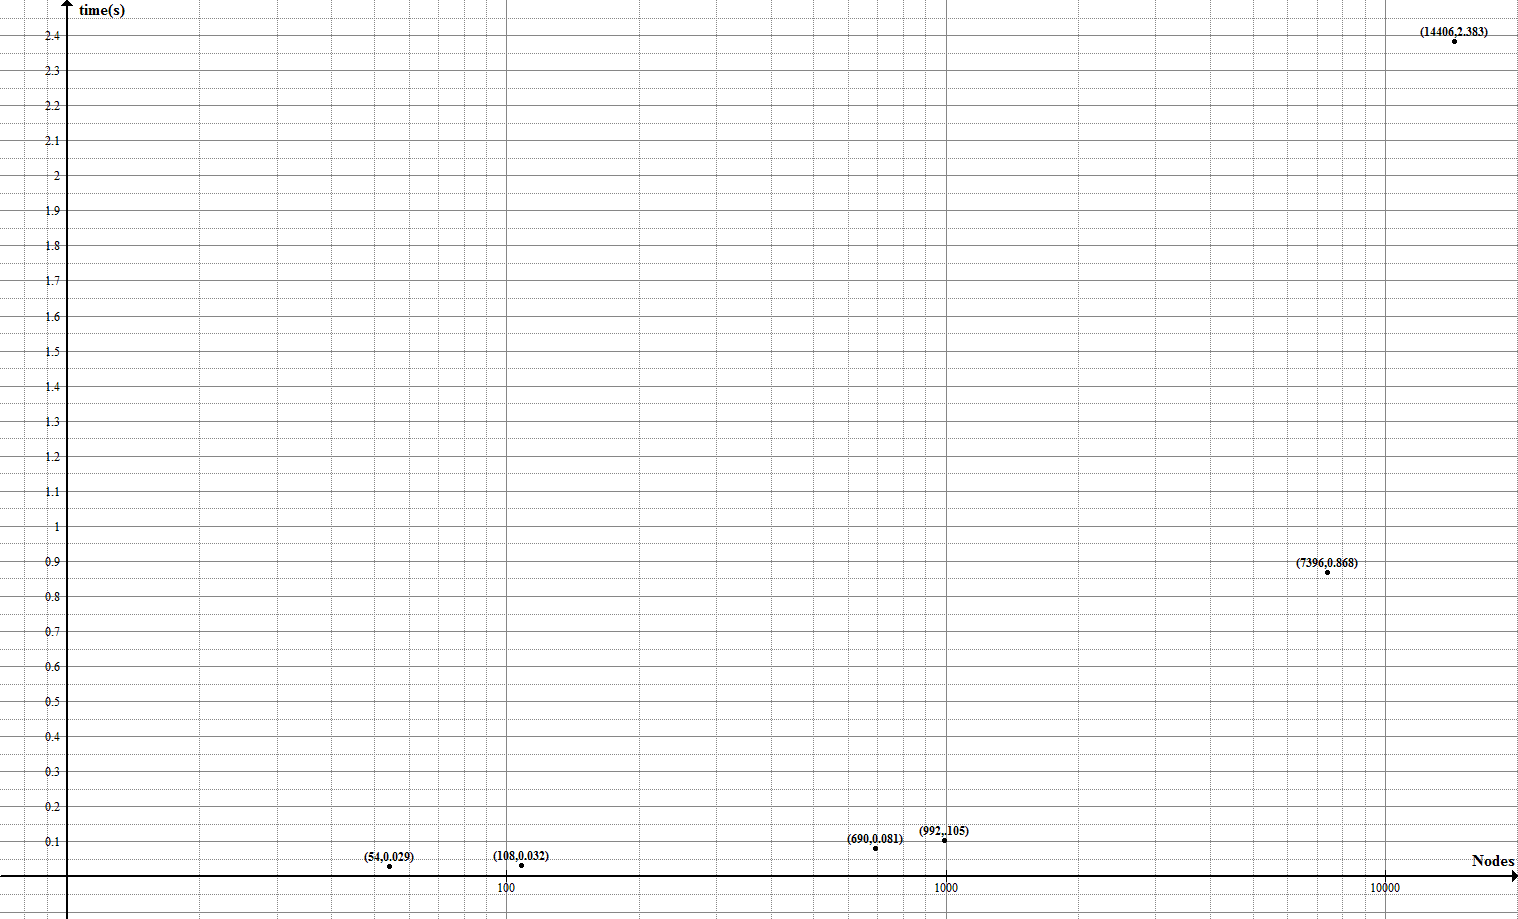
\includegraphics[width=0.3\textheight]{files/Adm.png}
		\caption{Admissible (Σχήμα ~\ref{fig:adm})}
	\end{minipage}
	\hspace{1cm}
	\begin{minipage}[b]{0.4\textwidth}
		\begin{flushright}
			\raggedright
			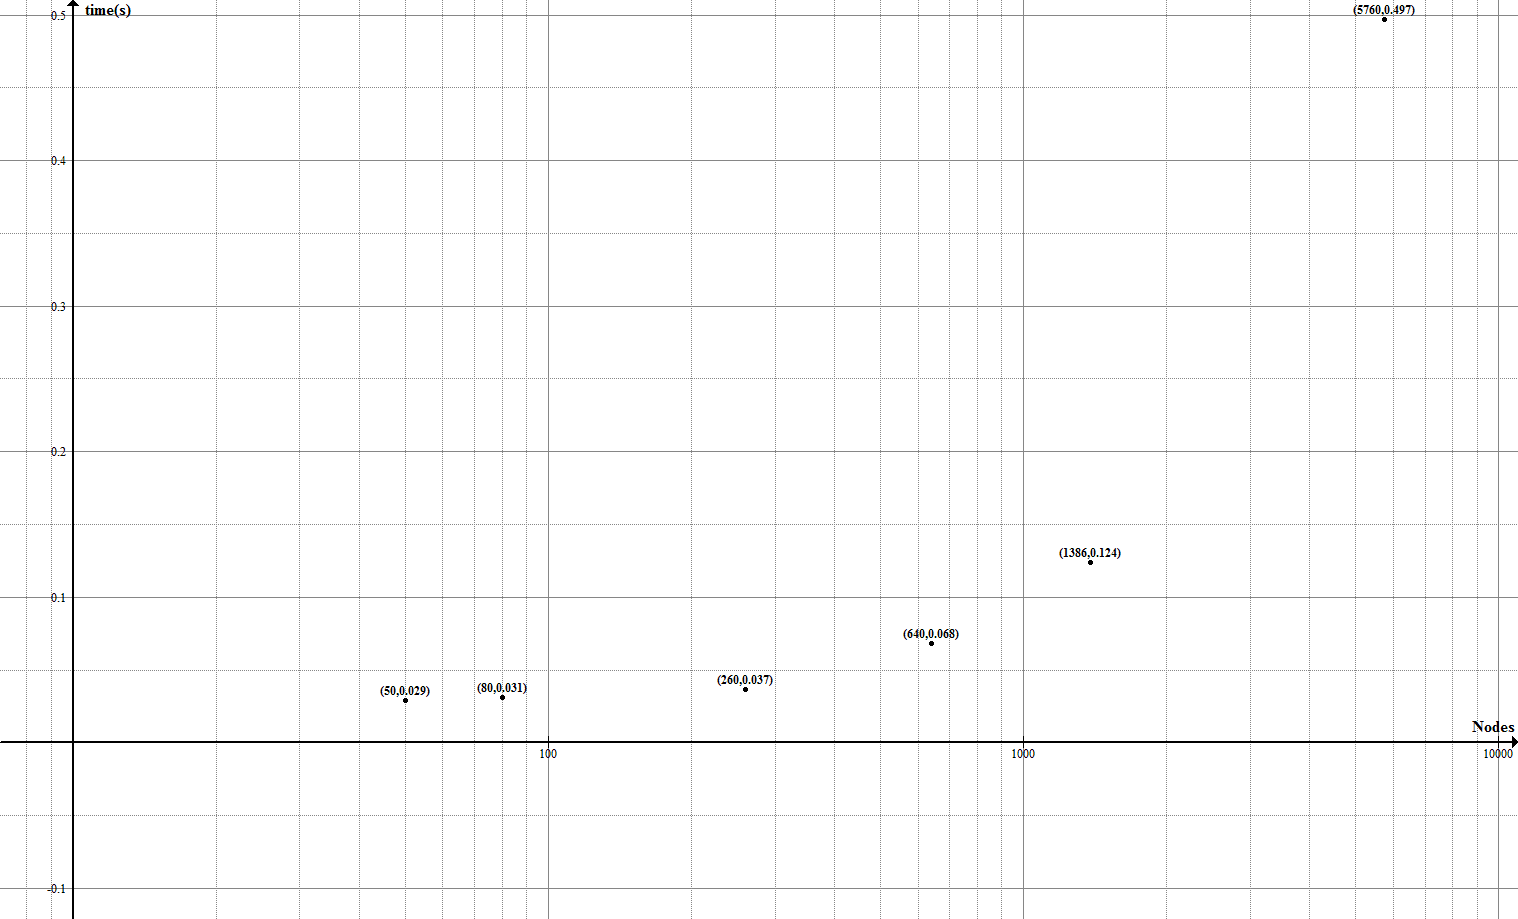
\includegraphics[width=0.3\textheight]{files/NonAdm.png}
			\caption{Non Admissible (Σχήμα ~\ref{fig:nonadm})}
		\end{flushright}
	\end{minipage}
\end{figure}

\begin{figure}[H]
	\centering
	\begin{minipage}{0.4\textwidth}
		\raggedleft
		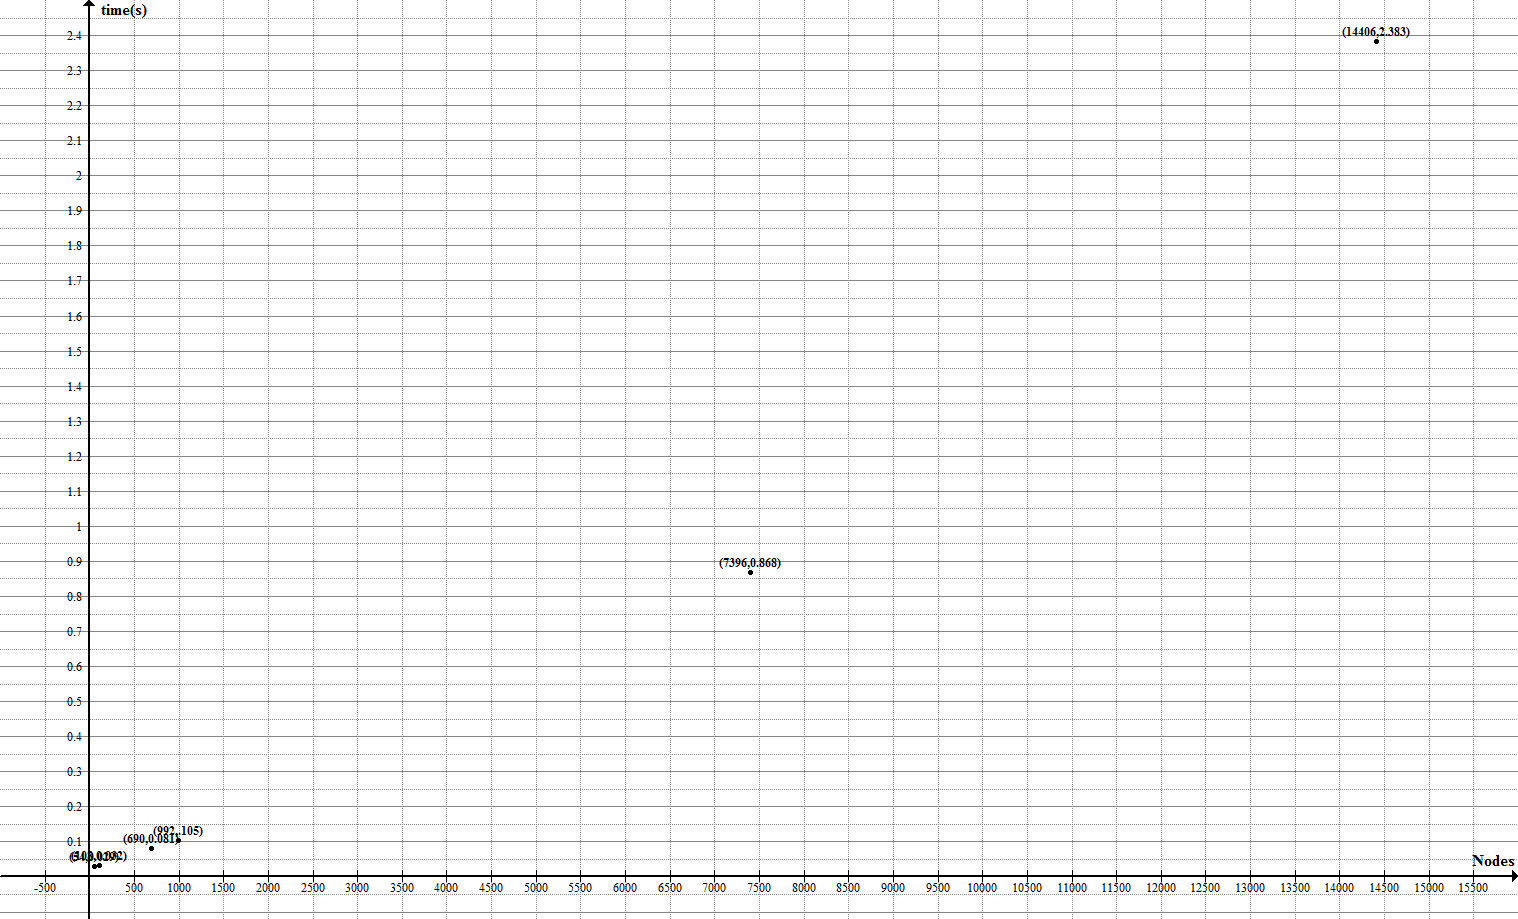
\includegraphics[width=0.3\textheight]{files/logAdm.png}
		\caption{Admissible (Σχήμα ~\ref{fig:logadm})}
	\end{minipage}
	\hspace{1cm}
	\begin{minipage}{0.4\textwidth}
		\raggedright
		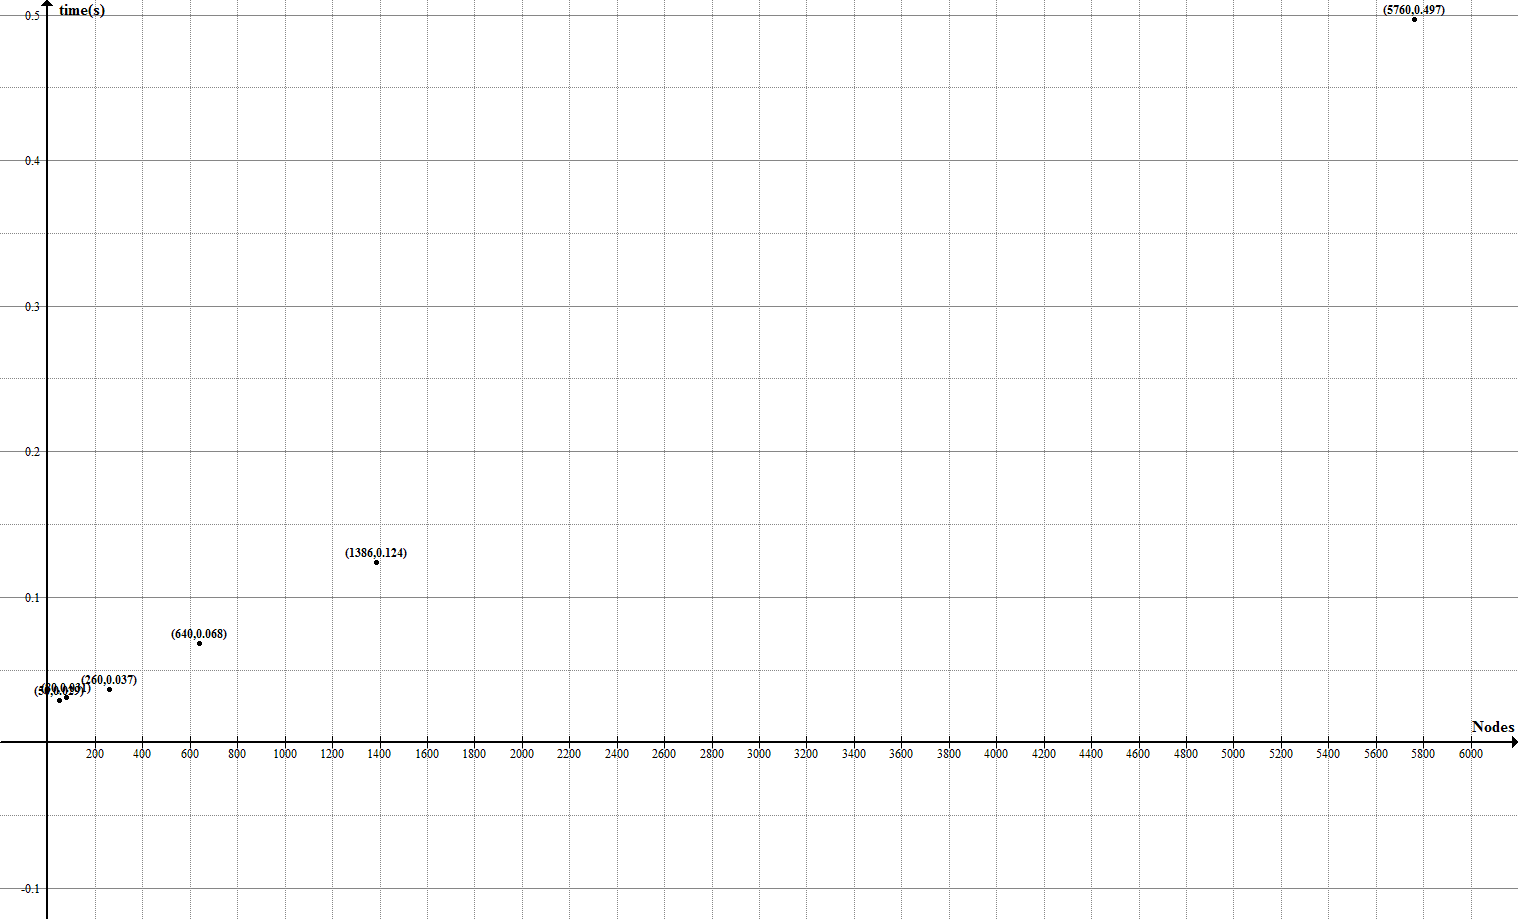
\includegraphics[width=0.3\textheight]{files/logNonAdm.png}
		\caption{Non Admissible (Σχήμα ~\ref{fig:lognonadm})}
	\end{minipage}
\end{figure}

%}}}

%{{{ Output examples

\subsection{Εκτύπωση βημάτων-συγκρούσεων-εναλλακτικών δρόμων σε παράδειγμα
εκτέλεσης}
\begin{figure}[H]
	\centering
	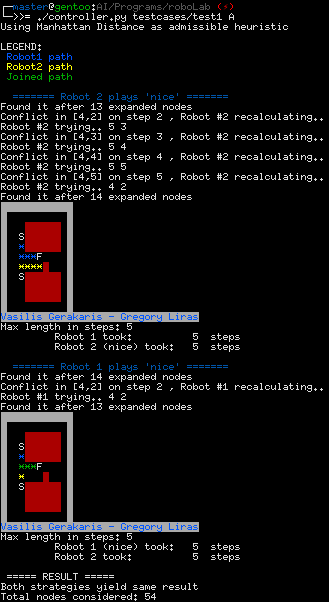
\includegraphics[scale=1]{files/test1.png}
	\caption{Tes{\kern0pt}tcase 1}
\end{figure}
\begin{figure}[H]
	\centering
	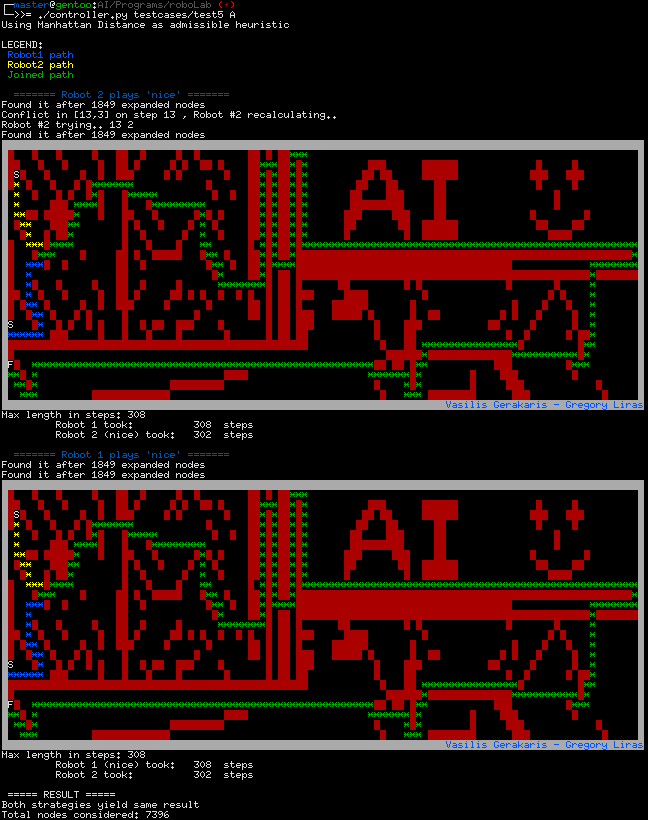
\includegraphics[width=0.9\textwidth]{files/test5.png}
	\caption{Tes{\kern0pt}tcase 5}
\end{figure}

%}}}

%{{{ Source code

\pagebreak
\subsection{Πηγαίος κώδικας}
\begin{itemize}
	\item
		Οι συναρτήσεις που καλούνται για την ανάγνωση της εισόδου:
		\inputminted[linenos,fontsize=\footnotesize,frame=leftline]{python}{files/inparser.py}

	\item
		Οι ευριστικές που χρησιμοποιούνται στον αλγόριθμο:
		\inputminted[linenos,fontsize=\footnotesize,frame=leftline]{python}{files/heuristics.py}

	\item
		Το κυρίως σώμα του A* :
		\inputminted[linenos,fontsize=\footnotesize,frame=leftline]{python}{files/astar.py}

	\item
		Οι συναρτήσεις που σχετίζονται με την εμφάνιση και τροποποίηση του χώρου
		καταστάσεων:
		\inputminted[linenos,fontsize=\footnotesize,frame=leftline]{python}{files/grids.py}

	\item
		Ο controller που καλεί τις παραπάνω συναρτήσεις για να παραχθεί το τελικό
		αποτέλεσμα:
		\inputminted[linenos,fontsize=\footnotesize,frame=leftline]{python}{files/controller.py}
\end{itemize}

%}}}

%{{{ Large figures

\begin{figure}[H]
	\centering
	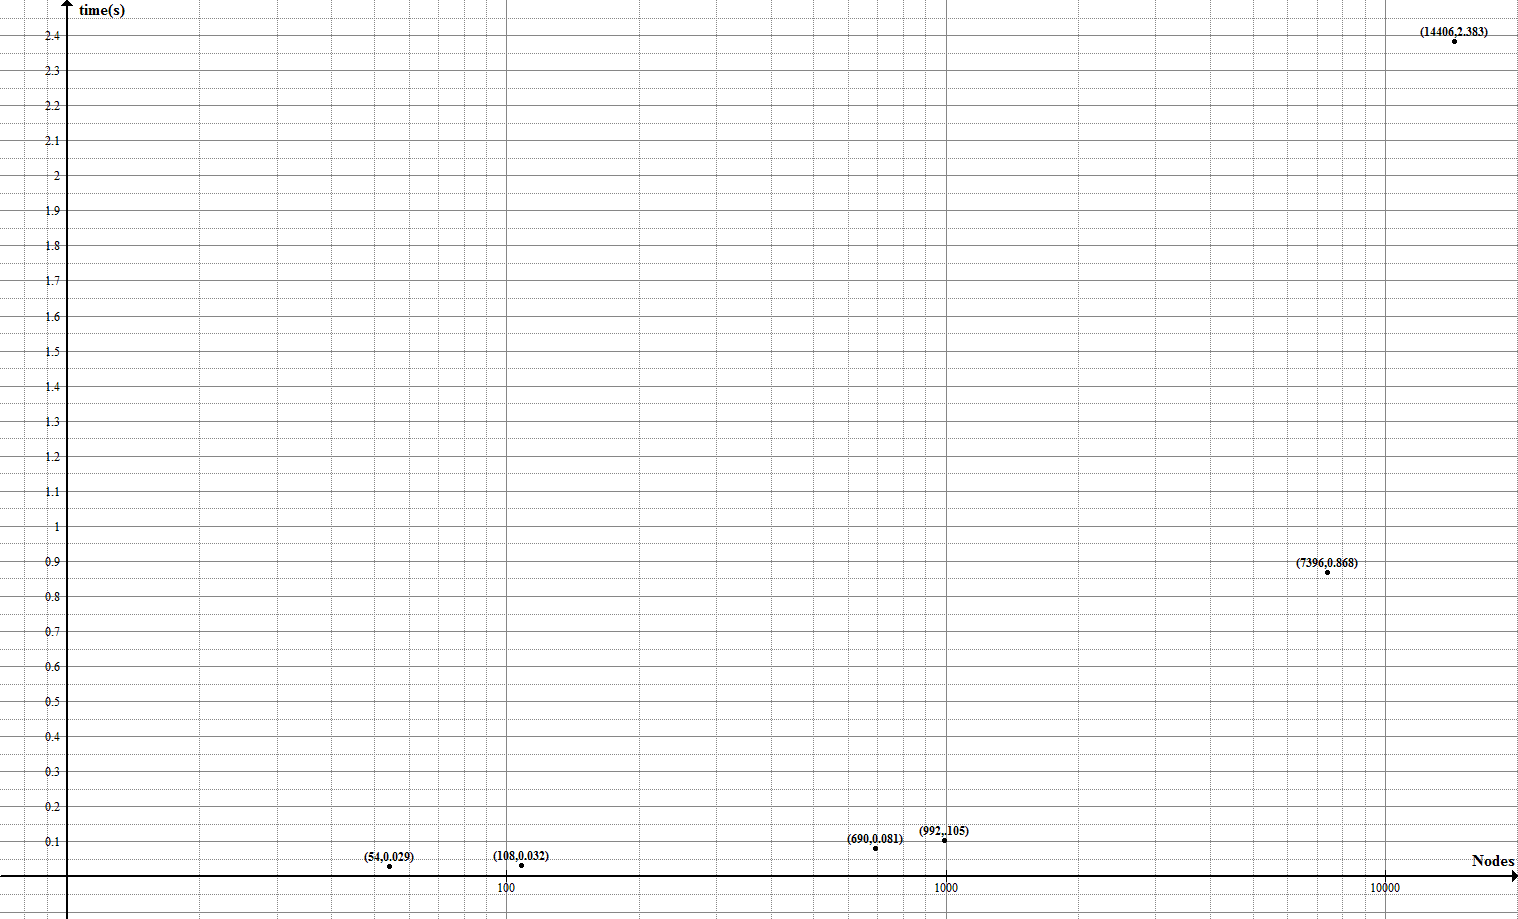
\includegraphics[width=\textheight,angle=90]{files/Adm.png}
	\caption{Admissible heuris{\kern0pt}tic}
	\label{fig:adm}
\end{figure}

\begin{figure}[H]
	\centering
	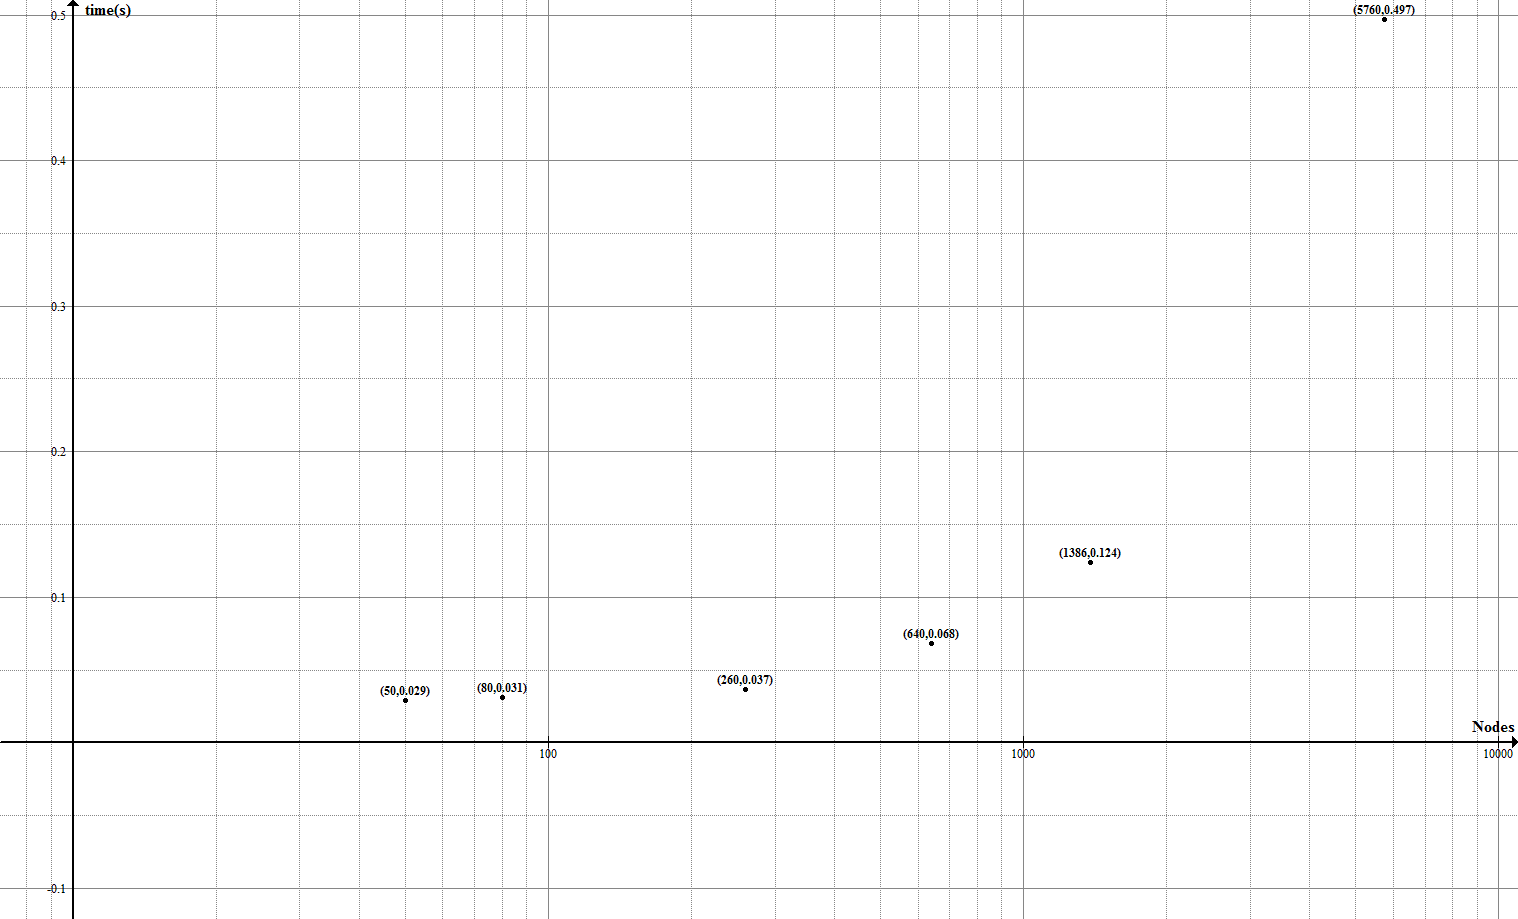
\includegraphics[width=\textheight,angle=90]{files/NonAdm.png}
	\caption{Admissible heuris{\kern0pt}tic}
	\label{fig:nonadm}
\end{figure}

\begin{figure}[H]
	\centering
	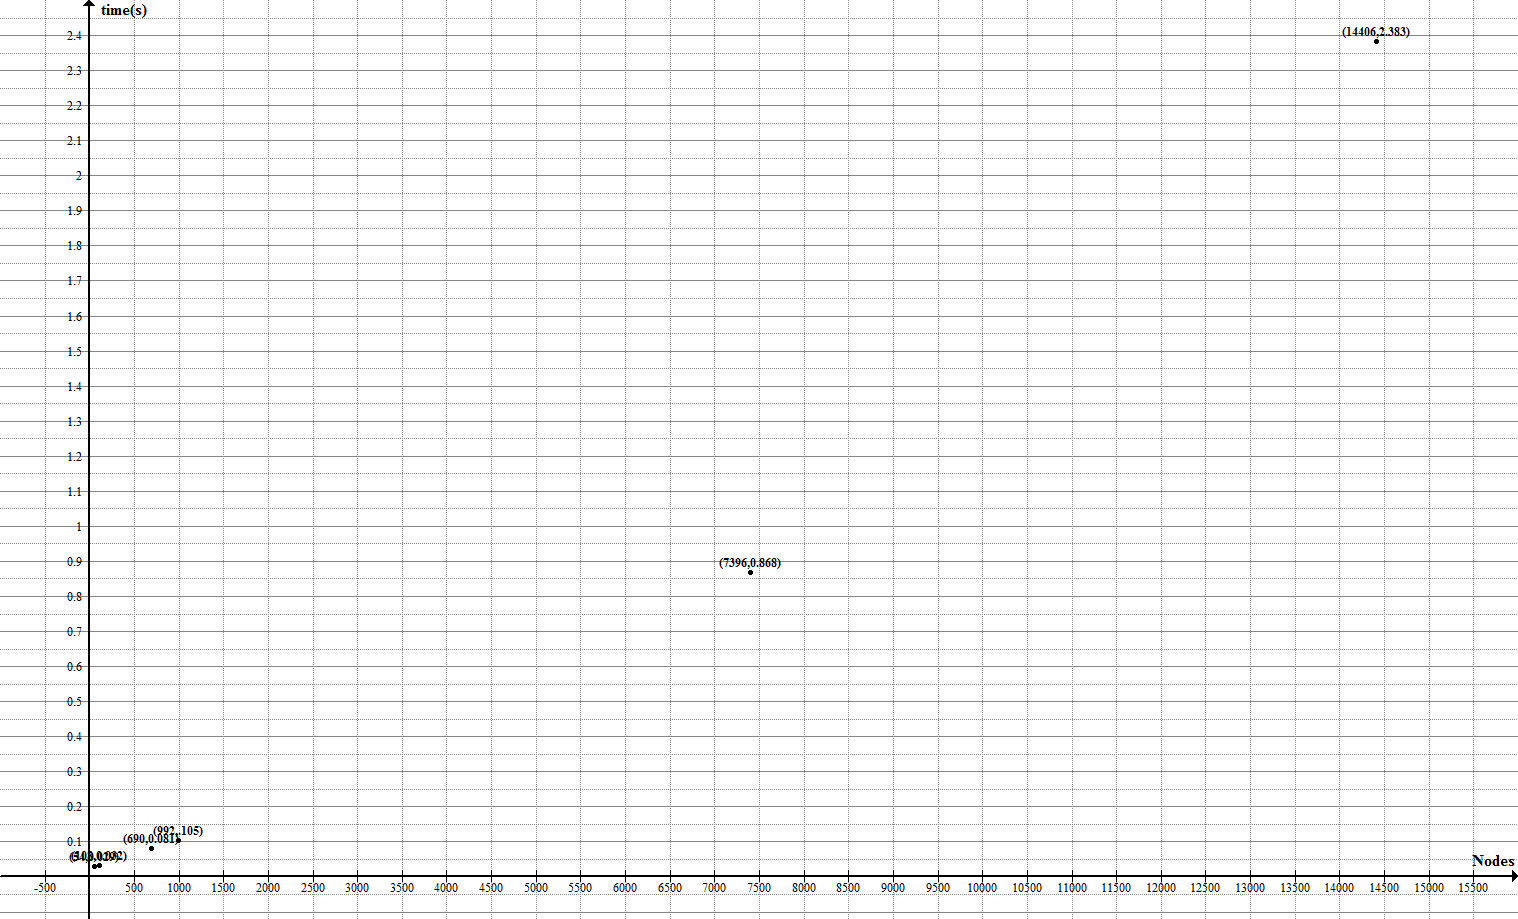
\includegraphics[width=\textheight,angle=90]{files/logAdm.png}
	\caption{Admissible heuris{\kern0pt}tic}
	\label{fig:logadm}
\end{figure}

\begin{figure}[H]
	\centering
	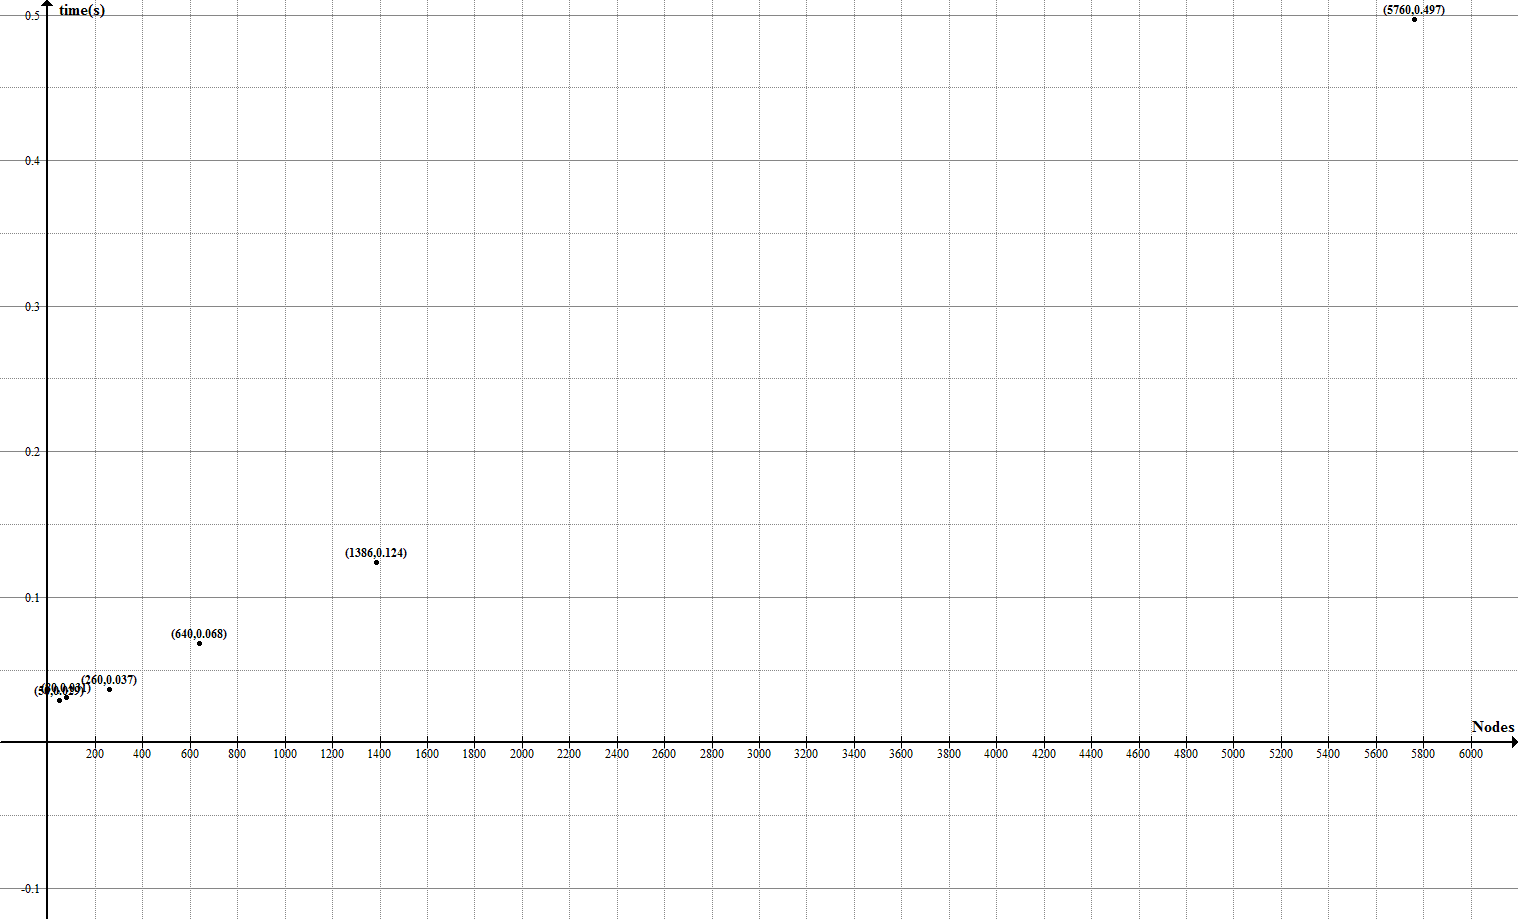
\includegraphics[width=\textheight,angle=90]{files/logNonAdm.png}
	\caption{Admissible heuris{\kern0pt}tic}
	\label{fig:lognonadm}
\end{figure}

%}}}
\end{document}
